% Generated by my modifications to the default Pandoc beamer template.
% Karl Browman has a tutorial about how to make Beamer sane:
% http://kbroman.wordpress.com/2013/10/07/better-looking-latexbeamer-slides/

% 12pt by default; handout if the handout template variable is defined
\documentclass[12pt,ignorenonframetext,]{beamer}

\newcommand{\q}[1]{``#1''} 
\usepackage{hyperref}
\usepackage{bm}
\usepackage{tikz}
\usetikzlibrary{matrix,decorations.pathreplacing,calc}
\usepackage{parnotes}
\usepackage{animate}
\usetheme{Madrid}
\usepackage{fontspec}
\usefonttheme{professionalfonts}
\usefonttheme{serif}
\setmainfont[
     Path = /usr/share/texmf-dist/fonts/opentype/google/roboto/,
     Extension      = .otf,
     UprightFont    = *-Regular,
     ItalicFont     = *-LightItalic,
     BoldFont       = *-Bold,
     BoldItalicFont = *-BoldItalic,
]{Roboto}

\DeclareMathOperator*{\argmin}{\arg\!\min}
\DeclareMathOperator*{\argmax}{\arg\!\max}

%\logo{
\includegraphics[width=0.25\textwidth]{IST_A_CMYK_POS.pdf}}

\usecolortheme{whale}

%\definecolor{foreground}{RGB}{255,255,255}
%\definecolor{background}{RGB}{24,24,24}
%\definecolor{title}{RGB}{107,174,214}
%\definecolor{gray}{RGB}{155,155,155}
%\definecolor{subtitle}{RGB}{102,255,204}
%\definecolor{hilight}{RGB}{102,255,204}
%\definecolor{vhilight}{RGB}{255,111,207}
%
%\setbeamercolor{titlelike}{fg=title}
%\setbeamercolor{subtitle}{fg=subtitle}
%\setbeamercolor{institute}{fg=gray}
%\setbeamercolor{normal text}{fg=foreground,bg=background}
%
%\setbeamercolor{item}{fg=foreground} % color of bullets
%\setbeamercolor{subitem}{fg=gray}
%\setbeamercolor{itemize/enumerate subbody}{fg=gray}
%\setbeamertemplate{itemize subitem}{{\textendash}}
%\setbeamerfont{itemize/enumerate subbody}{size=\footnotesize}
%\setbeamerfont{itemize/enumerate subitem}{size=\footnotesize}


\setbeameroption{hide notes}
\setbeamertemplate{note page}[plain]

% Don't show things we don't want to see
\beamertemplatenavigationsymbolsempty
%\hypersetup{pdfpagemode=UseNone} % don't show bookmarks on initial view

% Slide number in lower right
\definecolor{gray}{RGB}{155,155,155}
\setbeamertemplate{footline}{%
    
\includegraphics[width=2cm,trim={0 6cm 0 7cm},clip]{IST_A_CMYK_POS.pdf}%
    \hfill%
    \raisebox{5pt}{
    \makebox{%
        \color{gray}%
        \scriptsize%
        \insertframenumber\,/\,\inserttotalframenumber\kern1em%
    }%
    }%
\hspace*{5pt}}

% Space between paragraphs on notes page
\addtobeamertemplate{note page}{\setlength{\parskip}{12pt}}

% Color and shape of bullets
% \setbeamercolor{item}{fg=gray} 
% \setbeamercolor{subitem}{fg=gray}
% \setbeamercolor{itemize/enumerate subbody}{fg=gray}
\setbeamertemplate{itemize item}{{\textendash}}
\setbeamertemplate{itemize subitem}{{\textendash}}
\setbeamerfont{itemize/enumerate subbody}{size=\footnotesize}
\setbeamerfont{itemize/enumerate subitem}{size=\footnotesize}

\usepackage{amssymb,amsmath}
\usepackage{ifxetex,ifluatex}
\usepackage{fixltx2e} % provides \textsubscript
\ifxetex
  \usepackage{fontspec,xltxtra,xunicode}
  \defaultfontfeatures{Mapping=tex-text,Scale=MatchLowercase}
\else
  \ifluatex
    \usepackage{fontspec}
    \defaultfontfeatures{Mapping=tex-text,Scale=MatchLowercase}
  \else
    \usepackage[utf8]{inputenc}
  \fi
\fi

% Comment these out if you don't want a slide with just the
% part/section/subsection/subsubsection title:
\AtBeginPart{
  \let\insertpartnumber\relax
  \let\partname\relax
  \frame{\partpage}
}
\AtBeginSection{
  \let\insertsectionnumber\relax
  \let\sectionname\relax
  \frame{\sectionpage}
}
\AtBeginSubsection{
  \let\insertsubsectionnumber\relax
  \let\subsectionname\relax
  \frame{\subsectionpage}
}

\setlength{\parindent}{0pt}
\setlength{\parskip}{6pt plus 2pt minus 1pt}
\setlength{\emergencystretch}{3em}  % prevent overfull lines
\setcounter{secnumdepth}{0}
\title{Variational Mixture of Normalizing Flows}
\author{Guilherme Grijó Pen Freitas Pires}

\usepackage[
    backend=biber,
    style=authoryear,
    sortlocale=en_EN,
    natbib=true,
    url=false,
    doi=true,
    eprint=false
]{biblatex}
\newrobustcmd*{\parentexttrack}[1]{%
  \begingroup
  \blx@blxinit
  \blx@setsfcodes
  \blx@bibopenparen#1\blx@bibcloseparen
  \endgroup}

\AtEveryCite{%
  \let\parentext=\parentexttrack%
  \let\bibopenparen=\bibopenbracket%
  \let\bibcloseparen=\bibclosebracket}

\makeatother
\addbibresource{presentation.bib}

\AtBeginSection[]
{
    \begin{frame}
        \frametitle{Table of Contents}
        \tableofcontents[currentsection]
    \end{frame}
}
\begin{document}
{
\begin{frame}[plain,noframenumbering]
  \titlepage
  \begin{center}
    \centering
    Thesis to obtain the Master of Science degree in \\
    \textbf{Electrical and Computer Engineering} \\
    
\includegraphics[width=3cm]{IST_A_CMYK_POS.pdf}
  \end{center}
\end{frame}
}

\begin{frame}{Summary}
\protect\hypertarget{summary}{}

This work in one sentence:

\begin{itemize}
    \item The development of a mixture of \textbf{normalizing flows}
    and a (variational) training procedure for it.
\end{itemize}

\end{frame}

\hypertarget{introduction-and-motivation}{%
\section{Introduction and
Motivation}\label{introduction-and-motivation}}

\begin{frame}{Introduction and Motivation}
\protect\hypertarget{introduction-and-motivation-1}{}

\begin{itemize}
\onslide<1->{\item Deep generative models have been an active area of research, with promising
results.}
    \begin{itemize}
        \onslide<2->{\item Implicit distributions: Generative adversarial networks
            \autocites{GAN}, Variational Autoencoder \autocites{vaepaper}
            \begin{itemize} \item Don't allow explicit access to the density function \end{itemize}}
        \onslide<3->{\item Explicit distributions: Normalizing flows
            \autocites{shakir_nf}
            \begin{itemize} \item Allow explicit access to the density function \end{itemize}}
    \end{itemize}
\end{itemize}

\end{frame}

\begin{frame}{Introduction and Motivation}
\protect\hypertarget{introduction-and-motivation-2}{}

\begin{itemize}
\onslide<1->{\item This work}
    \begin{itemize}
        \onslide<2->{\item How to endow normalizing flows with discrete structure?}
        \onslide<3->{\item Or, how to endow mixture models with more expressiveness/flexibility?}
    \end{itemize}
\end{itemize}

\end{frame}

\begin{frame}{Outline}
\protect\hypertarget{outline}{}

\begin{itemize}
\onslide<1->{\item Introductory concepts on probabilistic modelling}
\onslide<2->{\item Variational Inference}
    \onslide<3->{\begin{itemize} \item The chosen method for optimizing the model proposed in this work \end{itemize}}
\onslide<4->{\item Normalizing Flows}
    \onslide<5->{\begin{itemize} \item The centerpiece of the proposed model \end{itemize}}
\onslide<6->{\item Variational Mixture of Normalizing Flows}
\onslide<7->{\item Experiments and results}
\onslide<8->{\item Conclusions and future work}
\end{itemize}

\end{frame}

\hypertarget{probabilistic-modelling}{%
\section{Probabilistic Modelling}\label{probabilistic-modelling}}

\begin{frame}{Probabilistic Modelling: Goal}
\protect\hypertarget{probabilistic-modelling-goal}{}

Given data, find the probability distribution (commonly referred to as
the \emph{model}) that is the closest possible approximation to the true
distribution of the data.

\end{frame}

\begin{frame}{Probabilistic Modelling: Goal}
\protect\hypertarget{probabilistic-modelling-goal-1}{}

Informally, via Bayes' Law:

\begin{align*}
    p(\mbox{hypothesis}|\mbox{data}) = \frac{p(\mbox{data}|\mbox{hypothesis})p(\mbox{hypothesis})}{p(\mbox{data})} \label{eq:bayes}.
\end{align*}

\pause

The goal of probabilistic modelling is to find the optimal hypothesis
that maximizes (some form of) this expression.

\end{frame}

\begin{frame}{Probabilistic Modelling: Hypothesis}
\protect\hypertarget{probabilistic-modelling-hypothesis}{}

There are infinite candidate distributions to model the data. In
practice, the scope is narrowed to a class of hypothesis.

\pause

\begin{itemize}[<+->]
    \item Parametric families: $p(\bm{x}|\bm\theta)$
    \item Particular factorizations: e.g. $p(\bm{x}) = \prod_i^N p(x_i|x_{i-1})$
    \item Latent variables: $p(\bm{x}) = \int p(\bm{x}, \bm{z}) d\bm{z}$\footnote<4->{In
    the case of discrete latent variables, the integral becomes a sum}
    \item All of the above, combined
\end{itemize}

\end{frame}

\begin{frame}{Probabilistic Modelling: Hypothesis}
\protect\hypertarget{probabilistic-modelling-hypothesis-1}{}

Example: Mixture Models.

\pause

A mixture model is defined as: \begin{align*}
    p(\bm{x}, \bm{z}) = p(\bm{x}|\bm{z}, \bm\theta) p(\bm{z})
\end{align*}

\pause

\centering

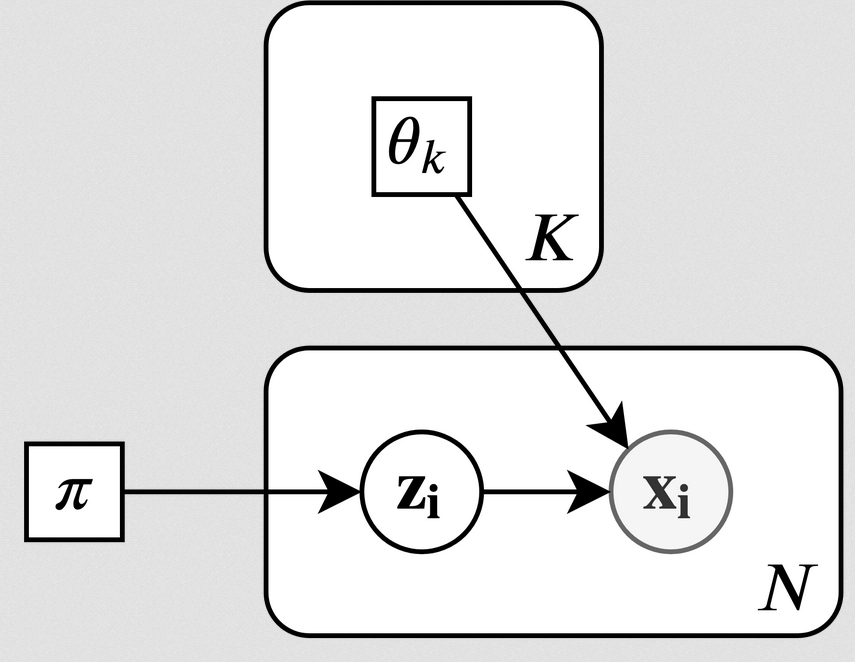
\includegraphics[width=0.5\textwidth]{figures/plate_diagram2.png}

\end{frame}

\begin{frame}{Probabilistic Modelling: Parameter Estimation}
\protect\hypertarget{probabilistic-modelling-parameter-estimation}{}

Given data \(\bm{x}\) and a parametric model \(p(\bm{x}| \bm\theta)\),
to estimate \(\bm\theta\):

\pause

Maximum-likelihood: \begin{align*}
\begin{cases}
    \bm{\hat\theta}_{ML} = \argmax_{\bm{\theta}} \mathcal{L}(\bm{\theta}),\\
    \mathcal{L}(\bm{\theta}) = p(\bm{x} | \bm{\theta})
\end{cases}
\end{align*}

\pause

Maximum a posteriori: \begin{align*}
\begin{cases}
    \bm{\hat\theta}_{MAP} = \argmax_{\bm{\theta}} p(\bm{\theta} | \bm{x}),\\
    p(\bm{\theta} | \bm{x}) = \frac{p(\bm{x} |\bm{\theta})p(\bm{\theta})}{p(\bm{x})}.
\end{cases}
\end{align*}

\end{frame}

\begin{frame}{Probabilistic Modelling: Inference}
\protect\hypertarget{probabilistic-modelling-inference}{}

Given data, \(\bm{x}\), and a model \(p(\bm{x}, \bm{z})\), one is
generally interested in finding the posterior:

\pause

\begin{align*}
    p(\bm{z}|\bm{x}) &= \frac{p(\bm{x}|\bm{z})p(\bm{z})}{p(\bm{x})} \\
                     &= \frac{p(\bm{x}|\bm{z})p(\bm{z})}{\int p(\bm{x}|\bm{z'})p(\bm{z'}) d\bm{z'}}.
\end{align*}

\pause

In general, the integral in the denominator is intractable. \onslide<4->

\(\to\) Approximate inference is required.

\end{frame}

\hypertarget{variational-inference}{%
\section{Variational Inference}\label{variational-inference}}

\begin{frame}{Variational Inference: Goal}
\protect\hypertarget{variational-inference-goal}{}

Variational Inference is one way of dealing with the intractability
previously described.

\pause

Given a \emph{variational} family \(q(\bm{z} ; \bm\lambda)\), find the
parameters \(\bm\lambda\) that minimze the Kullback-Leibler divergence
between \(q(\bm{z} ; \bm\lambda)\) and \(p(\bm{z}|\bm{x})\)

\end{frame}

\begin{frame}{Variational Inference: ELBO}
\protect\hypertarget{variational-inference-elbo}{}

\begin{align*}
\onslide<1->{KL(q||p) &= \int q(\bm{z}) \log\frac{q(\bm{z})}{p(\bm{z})} d\bm{z} \\}
\onslide<2->{&= \int q(\bm{z}) (\log q(\bm{z}) - \log p(\bm{z}|\bm{x})) d\bm{z} \\}
\onslide<3->{&= \int q(\bm{z}) (\log q(\bm{z}) - (\log p(\bm{x}, \bm{z}) - \log p(\bm{x}))) d\bm{z} \\}
\onslide<4->{&= \mathbb{E}_q [\log q(\bm{z})] - \mathbb{E}_q [\log p(\bm{x}, \bm{z})] + \log p(\bm{x})}
\end{align*}

\onslide<5->

Which yields the lower bound (ELBO): \begin{align*}
    ELBO(q) &= \mathbb{E}_q [\log p(\bm{x}, \bm{z})] - \mathbb{E}_q [\log q(\bm{z})] \\
            &= \mathbb{E}_q [\log p(\bm{x}|\bm{z})] + \mathbb{E}_q [\log p(\bm{z})] - \mathbb{E}_q [\log q(\bm{z})]
\end{align*}

\end{frame}

\hypertarget{normalizing-flows}{%
\section{Normalizing Flows}\label{normalizing-flows}}

\begin{frame}{Normalizing Flows: Change of Variables}
\protect\hypertarget{normalizing-flows-change-of-variables}{}

\onslide<1->{Given
\begin{align*}
\begin{cases}
    \bm{z} \sim p(\bm{z}) \\
    \bm{x} = g(\bm{z}; \bm\theta)
\end{cases}
\end{align*}}
\onslide<2->{then:
\begin{align*}
    f_X(\bm{x}) &= f_Z(g^{-1}(\bm{x};\bm\theta))\Big|\det\Big(\frac{d}{d\bm{x}}g^{-1}(\bm{x};\bm\theta)\Big)\Big| \\
    &= f_Z(g^{-1}(\bm{x};\bm\theta))\Big|\det\Big(\frac{d}{d\bm{z}}g(\bm{z};\bm\theta) \bigg{|}_{\bm{z} = g^{-1}(\bm{x};\bm\theta)}\Big)\Big|^{-1}
\end{align*}}

\onslide<3->{This can be optimize w.r.t. $\bm\theta$ so as to approximate
an arbitrary distribution}

\end{frame}

\begin{frame}{Normalizing Flows: Change of Variables}
\protect\hypertarget{normalizing-flows-change-of-variables-1}{}

\onslide<1->{The above can be useful if}
\begin{itemize}
    \onslide<2->{\item The base density has a closed form expression and is easy to sample from}
    \onslide<3->{\item The determinant of the Jacobian of $g$ is computationally cheap - not the case, in general}
    \onslide<4->{\item The gradient of the determinant of the Jacobian of $g$ w.r.t $\bm\theta$ is computationally cheap}
\end{itemize}

\end{frame}

\begin{frame}{Normalizing Flows: Change of Variables}
\protect\hypertarget{normalizing-flows-change-of-variables-2}{}

The framework of Normalizing Flows consists of composing several
transformations that fulfill the three listed conditions.

\end{frame}

\begin{frame}{Normalizing Flows: Affine Coupling Layer}
\protect\hypertarget{normalizing-flows-affine-coupling-layer}{}

An example of such a transformation is the Affine Coupling Layer
\autocites{real-nvp}.

\onslide<1->{Splitting $\bm{z}$ into $(\bm{z_1}, \bm{z_2})$,}
\onslide<2->{\begin{align*}
    \begin{cases}
    \bm{x_1} &= \bm{z_1} \odot \exp\big(s(\bm{z_2})\big) + t(\bm{z_2}) \\
    \bm{x_2} &= \bm{z_2}.
    \end{cases}
\end{align*}}
\onslide<3->{This transformation has the following Jacobian matrix:
\begin{align*}
    J_{f(z)} =
        \begin{tikzpicture}[decoration=brace, baseline=-\the\dimexpr\fontdimen22\textfont2\relax ]
            \matrix (m) [matrix of math nodes,left delimiter=[,right delimiter={]}, ampersand replacement=\&] {
                \mbox{\Large$\frac{\partial \bm{x_1}}{\partial \bm{z_1}}$} \& \mbox{\Large$\frac{\partial \bm{x_1}}{\partial \bm{z_2}}$} \\
                \mbox{\Large$\frac{\partial \bm{x_2}}{\partial \bm{z_1}}$} \& \mbox{\Large$\frac{\partial \bm{x_2}}{\partial \bm{z_2}}$} \\
            };
        \end{tikzpicture}
    =
        \begin{tikzpicture}[decoration=brace, baseline=-\the\dimexpr\fontdimen22\textfont2\relax ]
            \matrix (m) [matrix of math nodes,left delimiter=[,right delimiter={]}, ampersand replacement=\&] {
                \mbox{diag}\Big(\exp\big(s(\bm{z_2})\big)\Big) \& \mbox{\Large$\frac{\partial \bm{x_1}}{\partial \bm{z_2}}$} \\
                \mbox{\Large$\bm{0}$} \& \mbox{\Large$I$} \\
            };
        \end{tikzpicture}
\end{align*}
}

\end{frame}

\hypertarget{variational-mixture-of-normalizing-flows}{%
\section{Variational Mixture of Normalizing
Flows}\label{variational-mixture-of-normalizing-flows}}

\begin{frame}{VMoNF: Motivation}
\protect\hypertarget{vmonf-motivation}{}

\onslide<1->{How can we leverage the flexibility of normalizing flows, and endow it with
multimodal, discrete structure, like in a mixture model?}

\onslide<2->{Mixture of normalizing flows.}
\onslide<3->{
$\to$ Approximate inference is required.}

\end{frame}

\begin{frame}{VMoNF: Definition}
\protect\hypertarget{vmonf-definition}{}

Recall the ELBO: \begin{align*}
    ELBO(q) &= \mathbb{E}_q [\log p(\bm{x}|\bm{z})] + \mathbb{E}_q [\log p(\bm{z})] - \mathbb{E}_q [\log q(\bm{z})]
\end{align*}

\pause

Let the variational posterior \(q(z|x)\) be parameterized by a neural
network. We jointly optimize this objective, hence we learn the
variational posterior and the generative components simultaneously.

\end{frame}

\begin{frame}{VMoNF: Overview}
\protect\hypertarget{vmonf-overview}{}

\centering

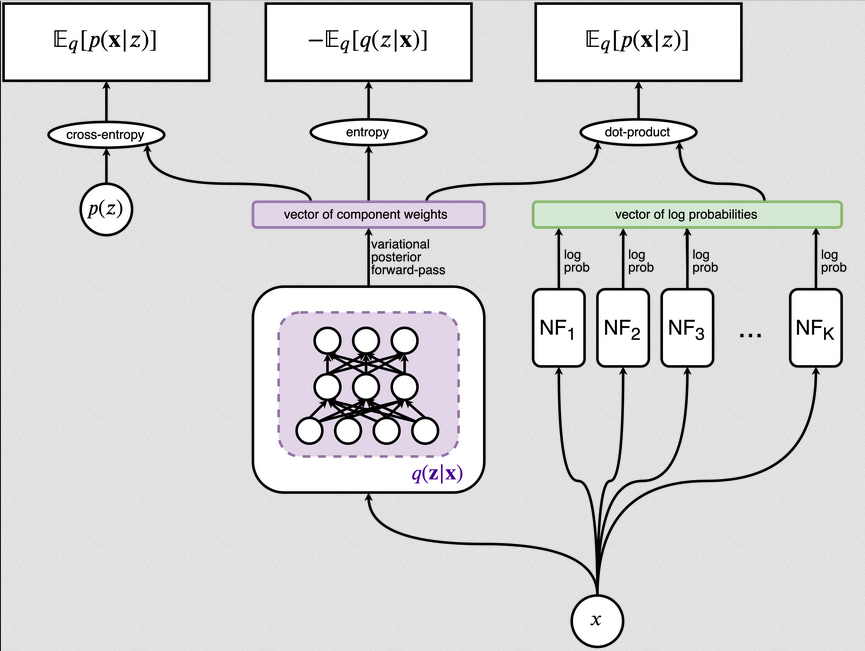
\includegraphics[width=0.7\textwidth]{figures/train_overview.png}

\end{frame}

\begin{frame}{VMoNF: Experiments - Pinwheel (5 wings)}
\protect\hypertarget{vmonf-experiments---pinwheel-5-wings}{}

\centering

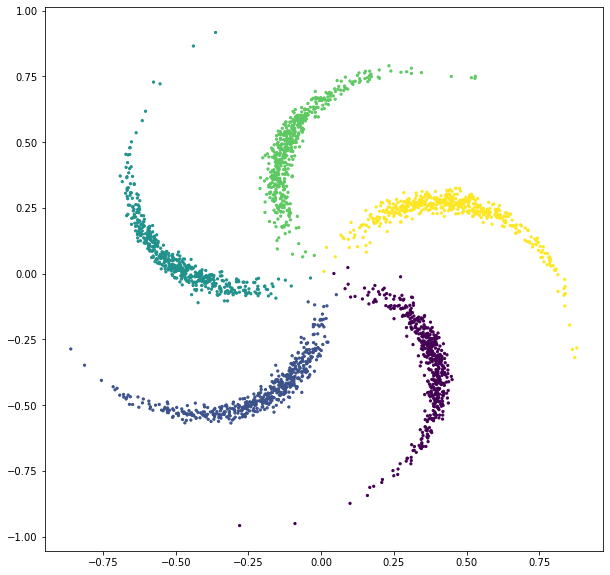
\includegraphics[width=0.475\textwidth]{figures/original_pinwheel.png}
\hfill
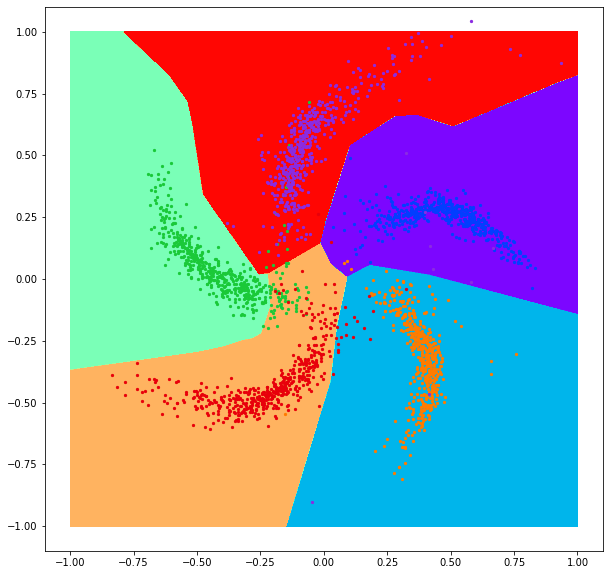
\includegraphics[width=0.475\textwidth]{figures/trained_pinwheel.png}

\end{frame}

\begin{frame}{VMoNF: Experiments - Pinwheel (3 wings)}
\protect\hypertarget{vmonf-experiments---pinwheel-3-wings}{}

\href{run:/home/colobas/dev/thesis/presentation/figures/animation/pinwheel.gif}{Trainining Animation}

\end{frame}

\begin{frame}{VMoNF: Experiments - 2 Circles}
\protect\hypertarget{vmonf-experiments---2-circles}{}

\centering

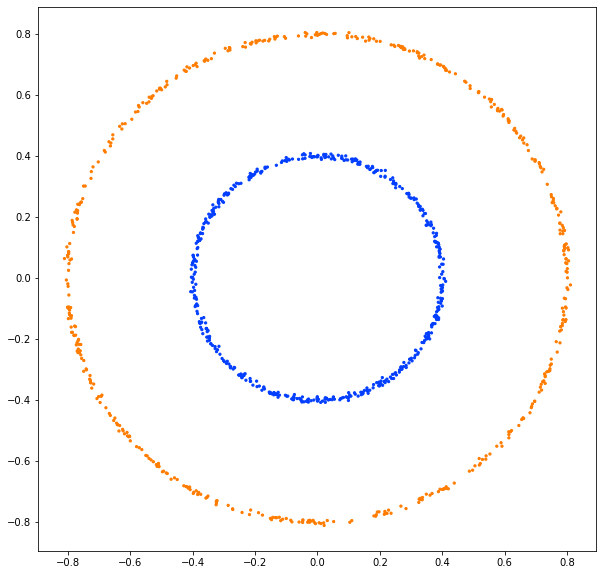
\includegraphics[width=0.475\textwidth]{figures/original_2_circles.png}
\hfill
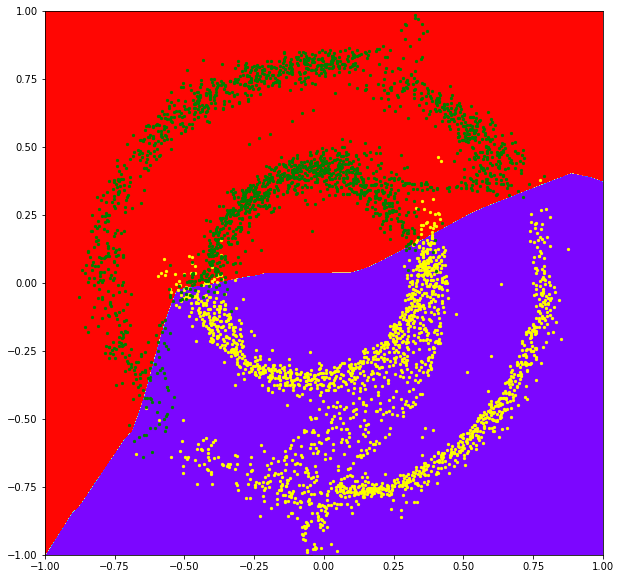
\includegraphics[width=0.475\textwidth]{figures/trained_2_circles_2.png}

\end{frame}

\begin{frame}{VMoNF: Experiments - 2 Circles (semi supervised)}
\protect\hypertarget{vmonf-experiments---2-circles-semi-supervised}{}

\centering

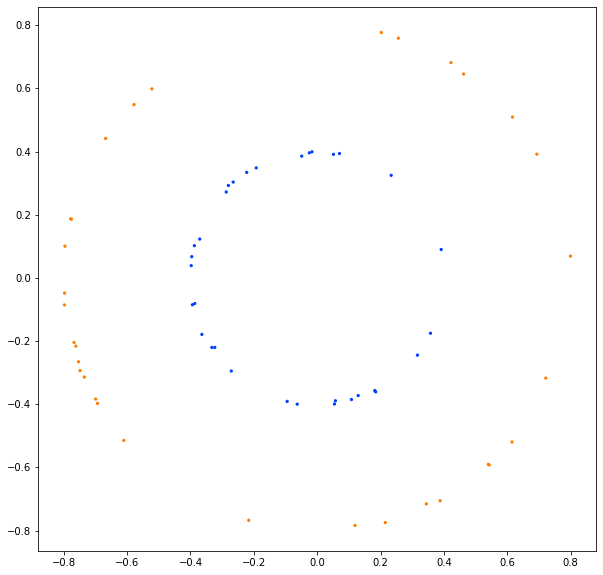
\includegraphics[width=0.475\textwidth]{figures/labeled_2_circles.png}
\hfill
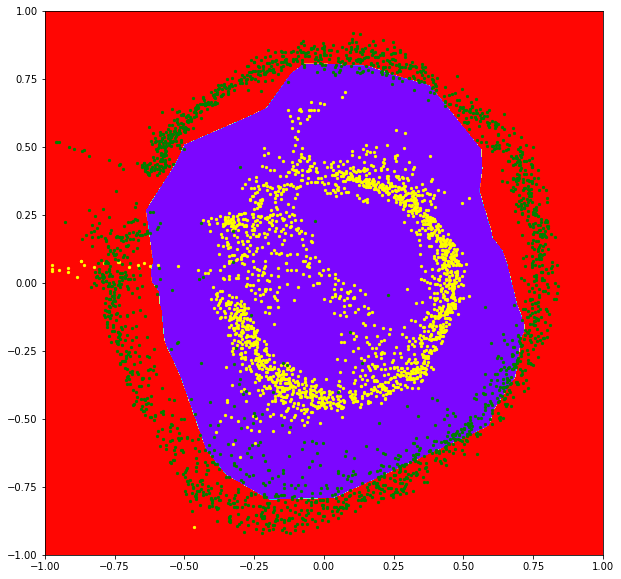
\includegraphics[width=0.475\textwidth]{figures/trained_2_circles_semisup.png}

Note: 32 labeled points, 1024 unlabeled points

\end{frame}

\begin{frame}{VMoNF: Experiments - MNIST}
\protect\hypertarget{vmonf-experiments---mnist}{}

\centering

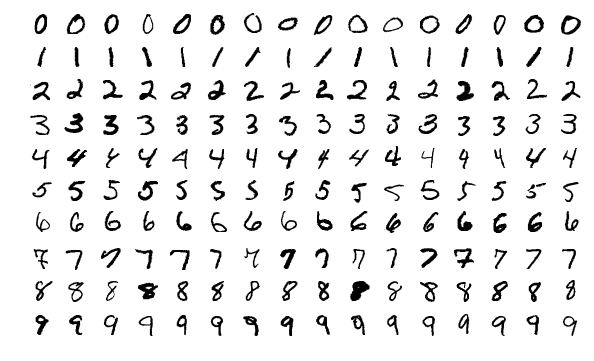
\includegraphics[width=0.7\textwidth]{figures/trained_mnist.png}

\end{frame}

\hypertarget{conclusions}{%
\section{Conclusions}\label{conclusions}}

\begin{frame}{Conclusions and Future Work}
\protect\hypertarget{conclusions-and-future-work}{}

\begin{itemize}
    \onslide<1->{\item Similar work is being pursued and published in prominent venues: \autocites{RAD}{semisuplearning_nflows}}
    \onslide<2->{\item Formally describe the reasons why the model fails in cases like the 2 circles $\to$ Topology}
        \onslide<3->{\begin{itemize} \item Investigate the effect of a consistency loss regularization term \end{itemize}}
    \onslide<4->{\item Weight-sharing between components}
    \onslide<5->{\item Balance between complexities}
    \onslide<6->{\item (Controlled) component anihilation}
\end{itemize}

\end{frame}

\begin{frame}{}
\protect\hypertarget{section}{}

Thank you!

\end{frame}

\end{document}
